\documentclass[sigconf]{acmart}
\settopmatter{printacmref=false} % Removes citation information below abstract
\renewcommand\footnotetextcopyrightpermission[1]{} % removes footnote with conference information in first column
\pagestyle{empty} % removes running headers
%%
%% \BibTeX command to typeset BibTeX logo in the docs
\AtBeginDocument{%
  \providecommand\BibTeX{{%
    \normalfont B\kern-0.5em{\scshape i\kern-0.25em b}\kern-0.8em\TeX}}}

\usepackage[linesnumbered,ruled]{algorithm2e}

\pagestyle{plain}
\graphicspath{ {../images/} }

\begin{document}


\title{Community Detection}

\author{Aitor Zubillaga}
\affiliation{%
  \institution{UPV/EHU}
  \country{}}
\email{zubillaga012@ikasle.ehu.eus}

\author{Julen Etxaniz}
\affiliation{%
  \institution{UPV/EHU}
  \country{}}
\email{jetxaniz007@ikasle.ehu.eus}


%%
%% By default, the full list of authors will be used in the page
%% headers. Often, this list is too long, and will overlap
%% other information printed in the page headers. This command allows
%% the author to define a more concise list
%% of authors' names for this purpose.

%%
%% The abstract is a short summary of the work to be presented in the
%% article.
\begin{abstract}
\%85 motibazioa, kontextua, proposamena, algoritmoa
\%15ondorioak esaldi bat

\end{abstract}


\maketitle

\section{Sarrera eta motibazioa}

Azken urteetan sare sozialek indar handia hartu dute. Arrazoi desberdin asko daude sare sozialen hazkundeen atzean, baina ukaezina da arrazoi nagusienetako bat, gure interesak partekatzen dituzten pertsonak aurkitzeko ematen dituzten erraztasunak direla [1]. Interesak edo erlazioak partekatzen dituzten pertsonen multzoei komunitate deitzen zaie. Pertsona multzo batean komunitateak aurkitzeko gai izan ezkero, posible da erabiltzaileari bere komunitate berdineko beste erabiltzaileei gogoko duten orrialdeen edo pertsonen gomendioak egitea, besteak beste. Hau horrela izanda, sare sozialen atzean dauden enpresek, interes handia erakutsi diote beraien erabiltzaileen artean komunitateak detektatzeko[2] modu egoki bat aurkitzeari. Komunitateak islatzeko orokorrean grafo egiturak erabiltzen dira, non pertsona edo erabiltzaile bakoitza nodo bat den. Komunitateak elkarri oso loturik dauden nodoen bidez adieraziko genituzke. Lotura hauek nodo arteko ertzak dira. Komunitate desberdineko kideen artean ere egongo dira arkuak baina askoz kantitate txikiagoetan.

\ref{fig:graph}. irudian ikus daiteke adibide bat. Komunitateak nodoen koloreekin eta formekin adierazita daude eta ikus daitekeen bezala komunitate bereko nodoen artean ertz asko daude. Bestalde, komunitate desberdinekoen artean oso gutxi.

\begin{figure}
    \centering
    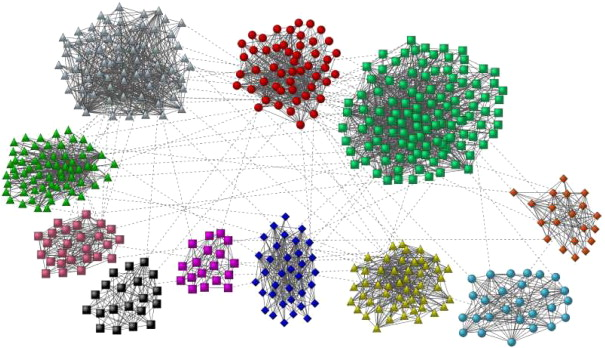
\includegraphics[width=\linewidth]{example.jpg}
    \caption{Komunitateak grafo batean}
    \label{fig:graph}
\end{figure}

Gure probleman, NIPS kongresuan publikatzen duten autoreen komunitateak aztertu nahiko ditugu. Zehazki, 2014 eta 2015 urteen bitartean, kongresu honetan eman diren elkarlan komunitate desberdinak aurkitu nahi ditugu. Komunitateak hainbat artikulu batera idatzi dituzten autoreek osatuko dituzte. Eta komunitate ezberdineko autoreen artean elkarlan gutxi egongo dira. 

Bilaketa espazioa $\{1,…,k\}^n$ da, non $k$ komunitateak eta $n$ autoreak diren. Autore bakoitza zein komunitatekoa den zehaztuko dugu kodeketa horrekin. Beraz, autoreak komunitatetan banatzen dituen partizio onena aurkitzea izango da helburua. Onena zein den jakiteko, helburu-funtzio egoki bat definitu beharko dugu.

Lan honen helburua grafoetan komunitateak aurkitzeko bi algoritmo diseinatu eta aztertzea da. Bata soluzio bakarrean oinarritutakoa izango da, eta bestea poblazionala. Lortutako emaitzak aztertzeko modularitatea erabiliko da. Modularitateak sare baten komunitate banaketaren egokitasuna neurtzen du. Banaketa egokia izango da komunitateen barruan ertz asko badaude, eta komunitate artean gutxi \cite{clauset2004finding}.

Izan bedi auzokidetasun matrizeko $A_{vw}$ elementua,  ertzen arteko pixuekin:

$$A_{vw} = \text{$v$ nodotik $w$ nodora doan ertzaren pisua}.$$

eta suposa dezagun erpinak komunitatetan banaturik daudela non $v$ ren komunitatea $c_v$ den. Beraz, komunitate berdinean erortzen diren pisuen frakzioa honakoa da 

$$\frac{\sum_{vw}A_{vw}\delta(c_v,c_w)}{\sum_{vw}A_{vw}}=\frac{1}{2m}\sum_{vw}A_{vw}\delta(c_v,c_w),$$

non $\delta$-funtzioa $\delta(i, j)$ en emaitza 1 den $i = j$ bada eta 0 bestela, eta $m = \frac{1}{2}\sum_{vw}A_{vw}$ grafoko ertzen pixuen batura den. Kantitate hau handia izango da sarearen banaketa onentzat, hau da, komunitateen barnean ertz asko badaude, baina hau ez da nahikoa banaketa ona den jakiteko. Adibidez, balio posible haundiena kasu tribial batean hartzen duelako, ertz guztiak komunitate berdinaren direnean, hau da, komunitateko bakarra dagoenean. Hau horrela, kantitate berdineko ausazko sare batengandik espero den balioa kentzen badiogu, neurri erabilgarri bat lortzen dugu.

Pixudun sare bateko $v$ erpin baten $k_{v}$ $graduak$ erpin honi lotutako ertzen pixuen batura da.

$$k_v = \sum_{w}A_{vw}.$$

Konexioak ausaz eginez baina erpinen graduak errespetatuz,  v eta w erpinen artean ertz bat existitzeko probabilitatea $k_{v}k_{w}/2m$ da. $Q$ modularitatea honela definitzen dugu

$$Q=\frac{1}{2m}\sum_{vw}\left[A_{vw}-\frac{k_vk_w}{2m}\right]\delta(c_v,c_w).$$

Komunitate barruko ertzen frakzioa ausazko sare batetik espero dezakegunaren desberdina ez bada, kantitate hau 0 izango da. 0 ez diren balioek ausazkotasunetik debiazioa errepresentatzen dute, eta praktikan 0.3 balioa sarearen komunitate estruktura ona denaren adierazgarria da. Beraz, gure helburua modularitatea maximizatzea izango da.

Gure algoritmoa sinplifikatzeko hurrengo bi kantitate definitko ditugu:

$$e_{ij}=\frac{1}{2m}\sum_{vw}A_{vw}\delta(c_v,i)\delta(c_w,j),$$

$i$ komunitatetik hasita $j$ komunitatea lotzen duten ertzen pisuen frakzioa, eta

$$a_i=\frac{1}{2m}\sum_{v}k_v\delta(c_v,i),$$

amaiera i komunitateko nodoetan duten pisuen frakzioa.
Beraz, $\delta(c_v,c_w) = \sum_i\delta(c_v,i)\delta(c_w,i)$, idatzi ezkero, hurrengoa dugu, (4) Eq.-tik

$$Q=\frac{1}{2m}\sum_{vw}\left[A_{vw}-\frac{k_vk_w}{2m}\right]\sum_i\delta(c_v,i)\delta(c_w,i) \\ $$

$$=\sum_i\left[\frac{1}{2m}\sum_{vw}A_{vw}\delta(c_v,i)\delta(c_w,i) \\
-\frac{1}{2m}\sum_{v}k_{v}\delta(c_v,i)\frac{1}{2m}\sum_{w}k_{w}\delta(c_w,i)\right] \\$$

$$=\sum_{i} (e_{ii} - a_i^2).$$

\section{Algoritmoen diseinua}

Soluzio bakarreko algoritmo moduan ILS bat inplementatu dugu. Algoritmo poblazional moduan GA-EDA algorimoa aukeratu dugu. Bi algoritmoek hasierako soluzioak lortzeko metodo eraikitzaile estokastiko bat erabiltzen dute, Louvain algoritmoan oinarritzen dena. Beraz, hasteko Louvain azalduko dugu eta ondoren besteak.

\subsection{Louvain}
Louvain algoritmoaren \cite{blondel2008fast} pausuak \ref{fig:louvain}. irudian ikus daitezke. Iterazio bakoitzak bi fase ditu: batean komunitateen aldaketa lokala bakarrik eginda modularitatea optimizatzen saiatzen da eta bestean, aurkitutako komunitateak agregatzen dira komunitateen sare berri bat sortzeko. Iterazio hauek modularitatea hobetzea posible ez den arte errepikatzen dira.

Community moduluko \texttt{generate\_dendogram} funtzioak komunitateak elkartzen ditu bakarrik hobetzen bada. Beraz, komunitate kopuru optimora iritsitakoan gelditu egiten da. Guri interesatzen zaigu emandako komunitate kopurua izatea, ez optimoa. 

Beraz, helburuko komunitate kopurura iritsitakoan algoritmoa geratzen dugu. Gainera, aldaketa batzuk egin ditugu komunitate kopurua gehiago jaitsi ahal izateko modularitatea asko txartu gabe. Horrela, $292$ komunitate ingurutik $279$ komunitate ingurura jaistea lortzen dugu.

Hala ere, honek ez du balio emandako komunitate kopurua $279$ baino txikiagoa bada. Izan ere, komunitateen artean ertzik ez dagoenean algoritmoa geratu egiten da. Hurrengo atalean komentatuko dugu nola lortu dugun txikitzea.

Community moduluko \texttt{best\_partition} edo gurea erabiltzen badugu antzeko arazoa daukagu, komunitate kopurua ezin da nahi adina jaitsi. Hori konpontzeko, \texttt{best\_fixed\_partition} funtzioa inplementatu dugu. Honek, lehenengo aurreko funtzioari deituko dio. Gero, soberan geratzen diren komunitate txikienak hartu eta guztiak komunitate berean elkartuko ditu. Izan ere, komunitateen artean konexiorik ez dagoenean, modularitate hobea lortzeko modurik onena komunitate txikienak elkartzea da, komunitate handiak eragin handiago baitute modularitatean eta hauek txartzeak beraz, asko jaisten du fitnessa. Komunitate txikienak non elkartu aukeratzeko, aukera guztiak aztertu eta onena aukeratzen da.

\begin{figure}
    \centering
    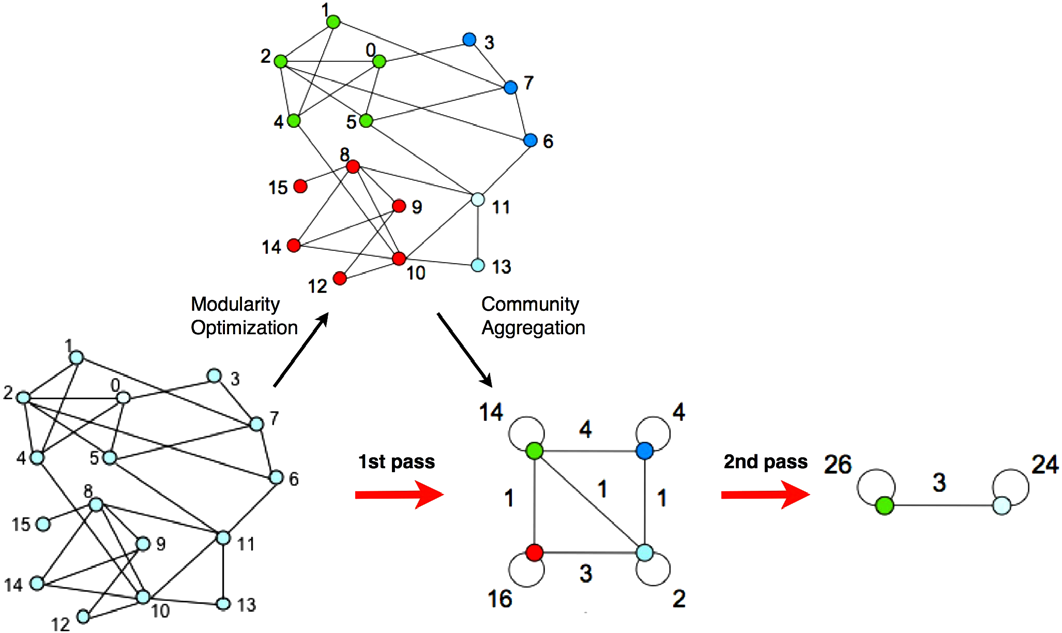
\includegraphics[width=\linewidth]{Louvain}
    \caption{Louvain}
    \label{fig:louvain}
\end{figure}

\subsection{ILS}
Iterated Local Search \cite{liu2020iterated} soluzio bakarreko algoritmoa inplementatu dugu . Hasierako soluzioa sortzeko Louvain eraikitzailea erabiltzen da. Ondoren, perturbazioak sartu, bilaketa lokala egiten da eta soluzioa eguneratzen da. Ikusi \ref{alg:ils}. algoritmoa.

\begin{algorithm}
    \SetKwInOut{Input}{Input}
    \SetKwInOut{Output}{Output}
    \Input{$local\_search$ bilaketa algoritmoa, $perturbation$ perturbazioa, $simmulated\_annealing$ onarpen-baldintza eta $stop\_criterion$ gelditzeko irizpidea}
    \Output{$s^*$ soluzioa}
    \While{$!stop\_criterion()$}{
        $s^* = perturbation(s^*)$
        
        $s = local\_search(s^*)$
        
        $s^* = simmulated\_annealing(s)$
    }
    \caption{ILS}
    \label{alg:ils}
\end{algorithm}

Perturbatzeko, lehenik soluzioan 2 komunitate ausaz hartu eta elkartu egiten dira, eta ondoren komunitate bat ausaz hartu eta bi zatitan banatzen da. Zati hauek ausaz aukeratzen dira. Funtzioak jasotako graduak, soluzioa zenbat aldiz perturbatuko den zehazten du. 

Behin perturbazioa sortuta, soluzio honen optimo lokala aurkituko da best first estrategia eta Swap ingurune funtzioa erabiliz. Emaitza eguneratzeko Simulated Annealing estrategia erabiliko dugu, emaitza txarragoak onartu ahal izateko. Gero eta tenperatura handiagoa, orduan eta probabilitate gehiago egongo da emaitza txarrak onartzeko. Hasierako tenperatura eta tenperatura egokitzeko modua aukeratu beharko ditugu.

\subsection{GA-EDA}
GA-EDA \cite{pena2004ga} populaziotan oinarritutako algoritmoa inplementatu dugu. Algoritmo honek Genetic Algorithms eta Estimation of Distribution Algorithms konbinatzen ditu. Bi algoritmo hauek antzekotasun asko dituzte, baina biak konbinatzean populazioetan dibertsitate gehiago eta emaitza hobeak lor daitezkeela ikusi dugu. Ikusi \ref{alg:ga_eda}. algoritmoa eta \ref{fig:ga_eda}. irudia.

\begin{figure}
    \centering
    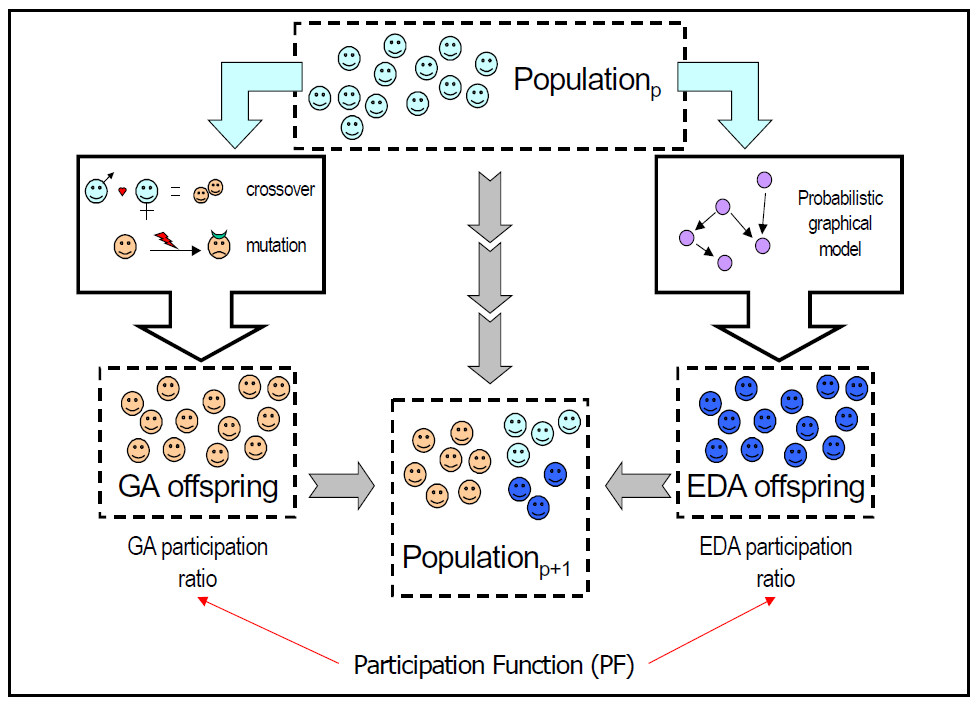
\includegraphics[width=\linewidth]{GA-EDA}
    \caption{GA-EDA}
    \label{fig:ga_eda}
\end{figure}

Hasteko, hasierako populazioa eraikiko dugu, ausaz edo moldatutako louvain heuristikoa erabiliz. Gero, hainbat iterazio egingo ditugu ebaluazio kopuru maximora iritsi arte. Iterazio bakoitzean pauso berdinak errepikatuko dira. Amaitzeko, populazioko soluzio onena itzuliko dugu.  

\begin{itemize}
    \item Selection eragiketan hainbat soluzio aukeratuko ditugu aurreko populaziotik. \texttt{best\_selection} aukeraketan beti soluzio onenak aukeratzen dira.  \texttt{roulette\_selection} aukeraketan soluzioen probabilitateak kalkulatzeko fitness balioa erabiltzen du. \texttt{rank\_selection} aukeraketan soluzioen probabilitateak kalkulatzeko ranking-eko posizioa erabiltzen da. \texttt{tournament\_selection} aukeraketan hainbat txapelketa egiten dira soluzioak ausaz aukeratuz.
    \item Crossover eragiketan aukeratutako soluzioak birkonbinatzen dira soluzio berriak sortzeko. \texttt{one\_point\_crossover} algoritmoan soluzioko puntu bat aukeratzen da. Puntu horretatik eskuinera dagoen soluzio zatia trukatzen da bi soluzioetan soluzio berriak sortuz.
    \item Mutation eragiketan, aurreko soluzioei mutazio bat egiten zaie probabilitate batekin. \texttt{bit\_mutation} eragiketan soluzioen posizio bakoitzaren balioa ausaz aldatzen da.
    \item Learning eragiketan, aukeratutako soluzioak erabilita eredu probabilistikoaren parametroak ikasten dira.
    \item Sampling eragiketan, ikasitako eredutik abiatuta soluzio berriak lagindu eta ebaluatzen dira.
    \item Update eragiketan, soluzio berrien eta aurrekoen artetik soluzio batzuk gordeko ditugu. \texttt{elistism\_update} eragiketak aurreko populazioko soluzio onena gordetzen du eta populazio berriko onenak. \texttt{elistism\_update} eragiketak aurreko populazioko eta populazio berriko soluzioak elkartzen ditu eta onenak aukeratzen ditu.
\end{itemize}

\begin{algorithm}
    \SetKwInOut{Input}{Input}
    \SetKwInOut{Output}{Output}
    \Input{$evaluate$, $select$, $learn$, $reproduce$, $sample$, $update$ eta $stop\_criterion$ operadoreak, $P_0$ hasierako populazioa}
    \Output{$s^*$ soluzioa}
    \While{$!stop\_criterion()$}{
        $f_t = evaluate(P_t)$
        
        $P^s_t = select(P_t, f_t)$
        
        $P^g_t = reproduce(P^s_t)$
        
        $P^e_t = sample(M_t)$
        
        $P_{t+1} = update(P_t, P^g_t, P^e_t)$
        
        $t = t + 1$
    }
    $s^* =$ Populazioko soluziorik onena
    \caption{GA-EDA}
    \label{alg:ga_eda}
\end{algorithm}

\section{Esperimentazioa}
Esperimentazioak bi fase izango ditu. Lehenengo fasean, ILS eta GA-EDA algoritmoen parametroak kalibratuko ditugu. Bigarren fasean, algoritmoak konparatuko ditugu 2 komunitatetik 100 komunitatera arte. Beti ere, jakiteko gure algoritmoak onak edo txarrak diren, RS baseline algoritmoa erabiliko dugu.

\subsection{Parametroak kalibratu}
Parametroak kalibratzeko Grid Search erabili dugu. Parametro garrantzitsuenetan hainbat balio posible definitu ditu eta beraien arteko konbinaketa denak probatu. Komunitate kopuruari dagokionez, muturreko kasuak bakarrik probatu ditugu, 2 eta 100 komunitate. 50 komunitaterekin ere probatu dugu baina antzekoak zirenez denbora aurrezteko kendu dugu. Gainerako parametroak gure ustez egokia den balio estatiko batean utzi ditugu. Izan ere, exekuzioak egiteko denbora asko behar da, eta luzea da parametro guztiak kalibratzea. 

Parametro aukera bakoitzerako $10^4$ ebaluazio eta 5 errepikapen egin ditugu. Errepikapen bakoitzeko fitness eta denbora balioaekin batazbestekoak kalkulatu ditugu. Fitness-en batazbesteko balioekin heatmap motako grafikak atera ditugu.

Ikusi \ref{fig:heatmap}. irudia.

\begin{figure}
    \centering
    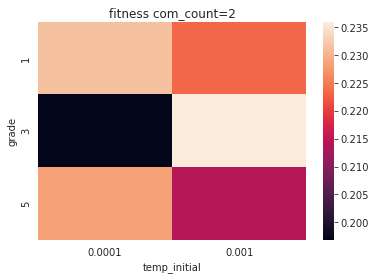
\includegraphics[width=\linewidth]{heatmap}
    \caption{Heatmap}
    \label{fig:heatmap}
\end{figure}

ILS algoritmoan komunitate kopuru bakoitzerako 6 parametro konbinazio probatu ditugu. Zehazki, perturbazio gradurako $\{1, 3, 5\}$ balioak eta simmulated annealing-en hasierako tenperaturarako $\{0.0001, 0.001\}$. Tenperatura eguneratzeko $0.9$ balioarekin bidertzen dugu beti. Bi komunitate kopuruetarako emaitza onena $3$ eta $0.001$ parametroekin lortu ditugu. Beraz, esperimentazioaren hurrengo faserako parametro horiek erabiliko ditugu.

GA-EDA algoritmoan, berriz, 4 parametro konbinazio probatu ditugu. Populazio tamainarako $\{30, 40\}$ eta aukeraketa tamainarako $\{15, 20\}$. Komunitate kopurua 2 denean, $30$ eta $15$ balioekin lortzen da fitness altuena. 100 komunitaterekin onena ez den arren, denak antzekoak dira. Gainera, denbora aldetik azkarrena da, soluzio kopurua txikiagoa delako. Ondorioz, parametro horiek erabiliko ditugu konparaketan.

\subsection{Algoritmoak konparatu}
Hiru algoritmoen konparaketa egiteko, komunitate kopuru bakoitzerako $10^4$ ebaluazio eta 5 errepikapen egin ditugu. Guztira 11 komunitate kopuru desberdin probatu ditugu, $2, 10, 20, ..., 100$. Emaitzekin boxplot motako grafikak atera ditugu, x ardatzean komunitate kopurua jarriz.

Ikusi \ref{fig:boxplot_fitness}. eta \ref{fig:boxplot_time} irudiak.

\begin{figure}
    \centering
    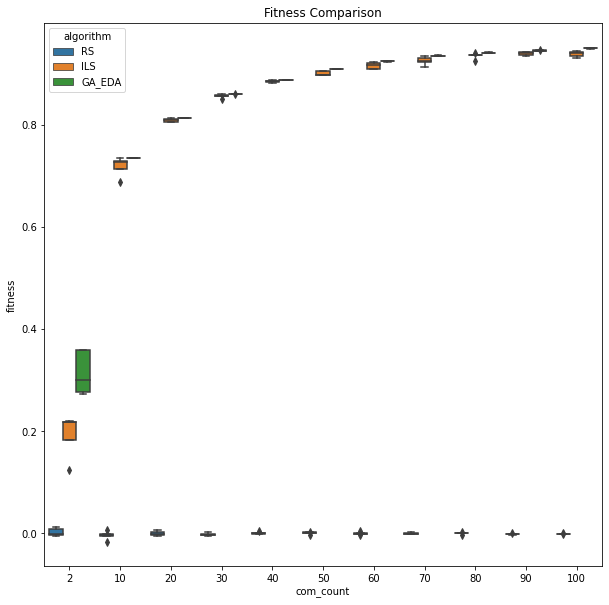
\includegraphics[width=\linewidth]{boxplot_fitness}
    \caption{Boxplot Fitnness}
    \label{fig:boxplot}
\end{figure}

\begin{figure}
    \centering
    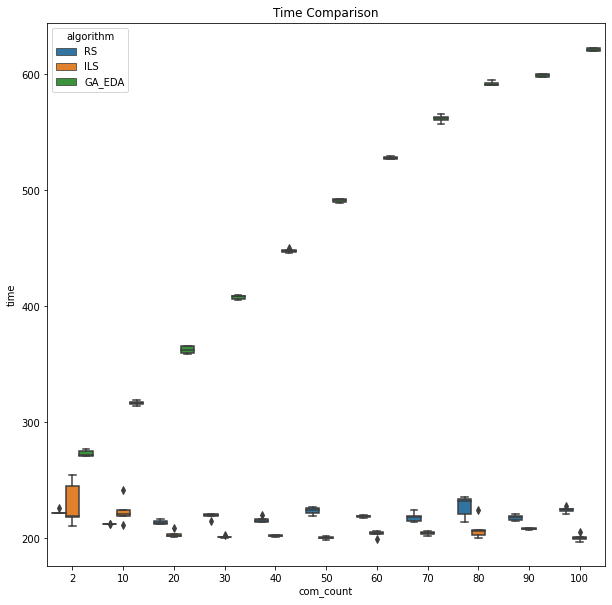
\includegraphics[width=\linewidth]{boxplot_time}
    \caption{Boxplot Time}
    \label{fig:boxplot}
\end{figure}

\section{Ondorioak}
\%15 motibazioa
\%85 azaldu proposamena + experimentuak + future work + limitations

\bibliographystyle{ACM-Reference-Format}
\bibliography{community}

\end{document}
\endinput
